\chapter{Choice of metrics}
\label{chap:metric}

\section{Venues metrics}

Before being able to compare set of venues, we need a distance function between
two venues, where venues are points in the feature space described in
\autoref{tab:venuefeatures} \vpageref{tab:venuefeatures}.

We evaluate the following metrics:
\begin{itemize}
	\item Euclidean norm
	\item Information Theoretic Metric Learning
	\item Gradient Boosted Large Margin Nearest Neighbor
	\item Euclidean norm in a 2D space reduced by t-SNE
\end{itemize}		
As well as two baselines:
\begin{itemize}
	\item $d_A$ where $A$ is a diagonal matrix with random coefficients in
		the range $[2, 20]$.
	\item Random ordering of venues. It is not a metric but because we
		only evaluate ranking instead of distances themselves that is
		enough.
\end{itemize}		
On two tasks:
\begin{enumerate}
	\item finding venue of the same brand in another city.
	\item finding venue of the same category in another city.
\end{enumerate}		

Evaluation is not straightforward as there are no easily available ground truth
indicating whether a given venue is close to another one or not. Thus we had to
rely on indirect information.

For the first task, we start by looking at common substrings in the name of venues
in Paris and Barcelona, keeping those that were company name and not mere
generic terms like \emph{park} or \emph{hotel}. We selected \emph{Starbucks} and
\emph{McDonald's} as they are ubiquitous and unambiguous. Then for each of
them in one city, we ranked all venues from the other city by how close they
are from this query and select the first one that was of the same brand. The
closest this first rank is the one, the better the metric. The results are
shown in \autoref{fig:brand}.

\begin{figure}[h]
        \centering
        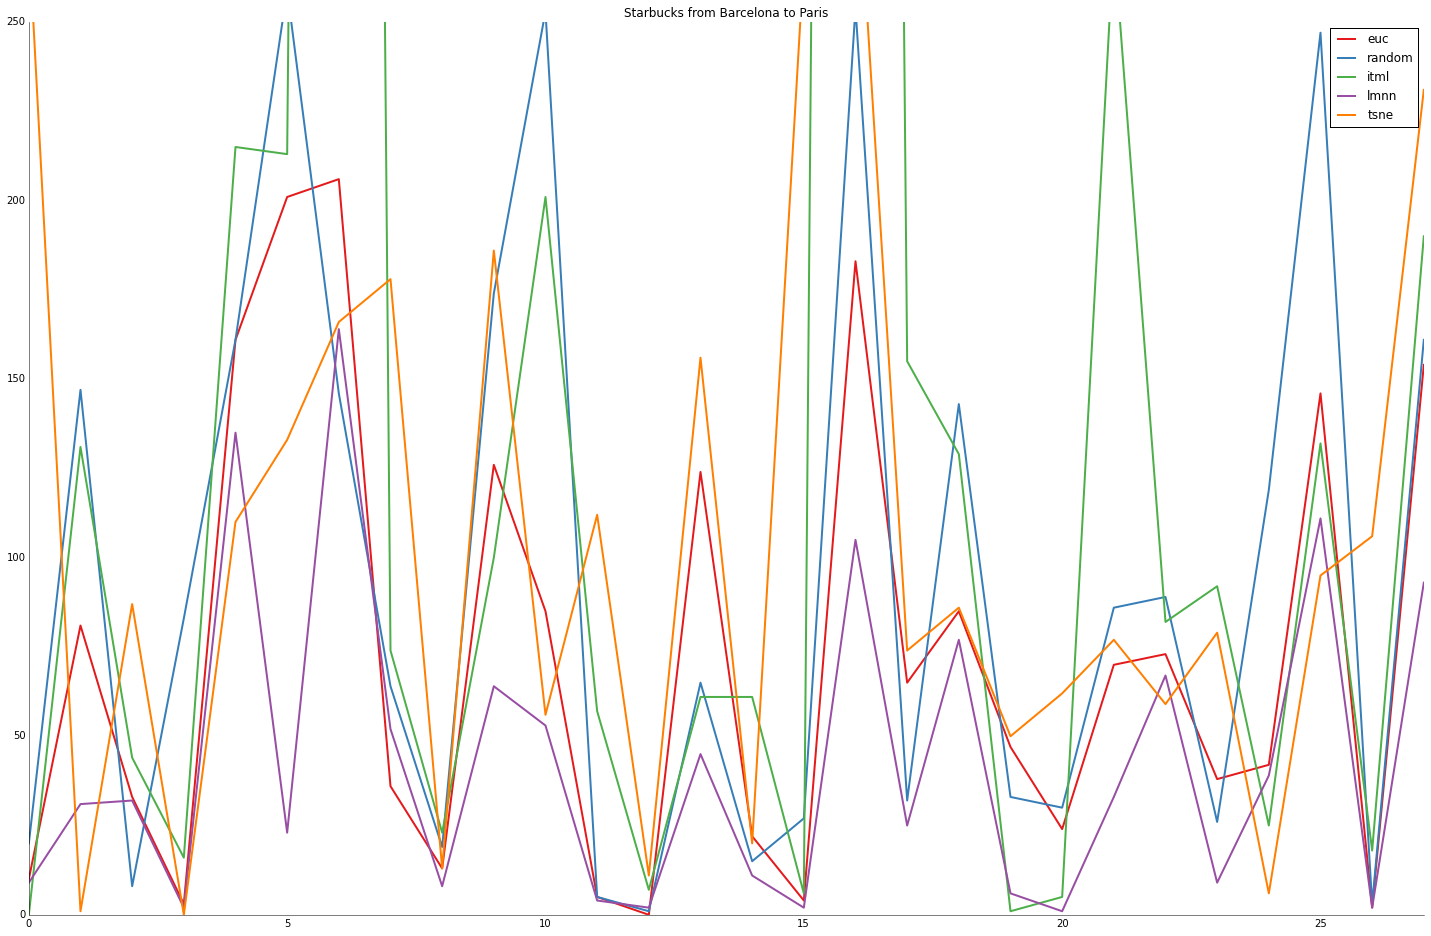
\includegraphics[width=\linewidth]{starbuck_barca_to_paris}
        \caption{How far is the first Starbucks in Paris when selecting a
        Starbucks in Barcelona}
        \label{fig:brand}
\end{figure}

The second task is more general. Each venue is assigned a hierarchical category
by Foursquare\footnote{The tree can be seen on their website:
\href{https://developer.foursquare.com/categorytree}{%
\url{developer.foursquare.com/categorytree}}.}. We restrict ourselves
to two levels, meaning that one venue can be a \emph{French Restaurant
$\rightarrow$ Food} and another one \emph{Airport $\rightarrow$ Travel
\& Transport}. We repeat the same sorting procedure but this time, we expect
venues of the same sub category to be first, followed by other venues of the
same top category and then the rest. To measure how well metrics achieved such
ranking, we use \methodname{Normalised Discounted Cumulative Gain}
\autocite{IREvaluation07}. The gain is a measure of relevance. We arbitrarily
choose $rel_i=1$ when the sub category of two venues matches, $rel_i=0.4$ when
only top category matches and $rel_i=0$ if they were not related at all. We
accumulate them (or sum them) but discount results that came too late with \[
\mathrm{DCG} = \sum_{i=1} \frac{ 2^{rel_{i}} - 1 }{ \log_{2}(i+1)} \]
Finally we normalized by the result of a perfect ordering to have scores
between $0$ and $1$, which allow direct comparison. The score of each metric
for each venue is showed in \autoref{fig:category}~\vpageref{fig:category}.

\begin{figure}[h]
    \begin{subfigure}[b]{\textwidth}
        \centering
        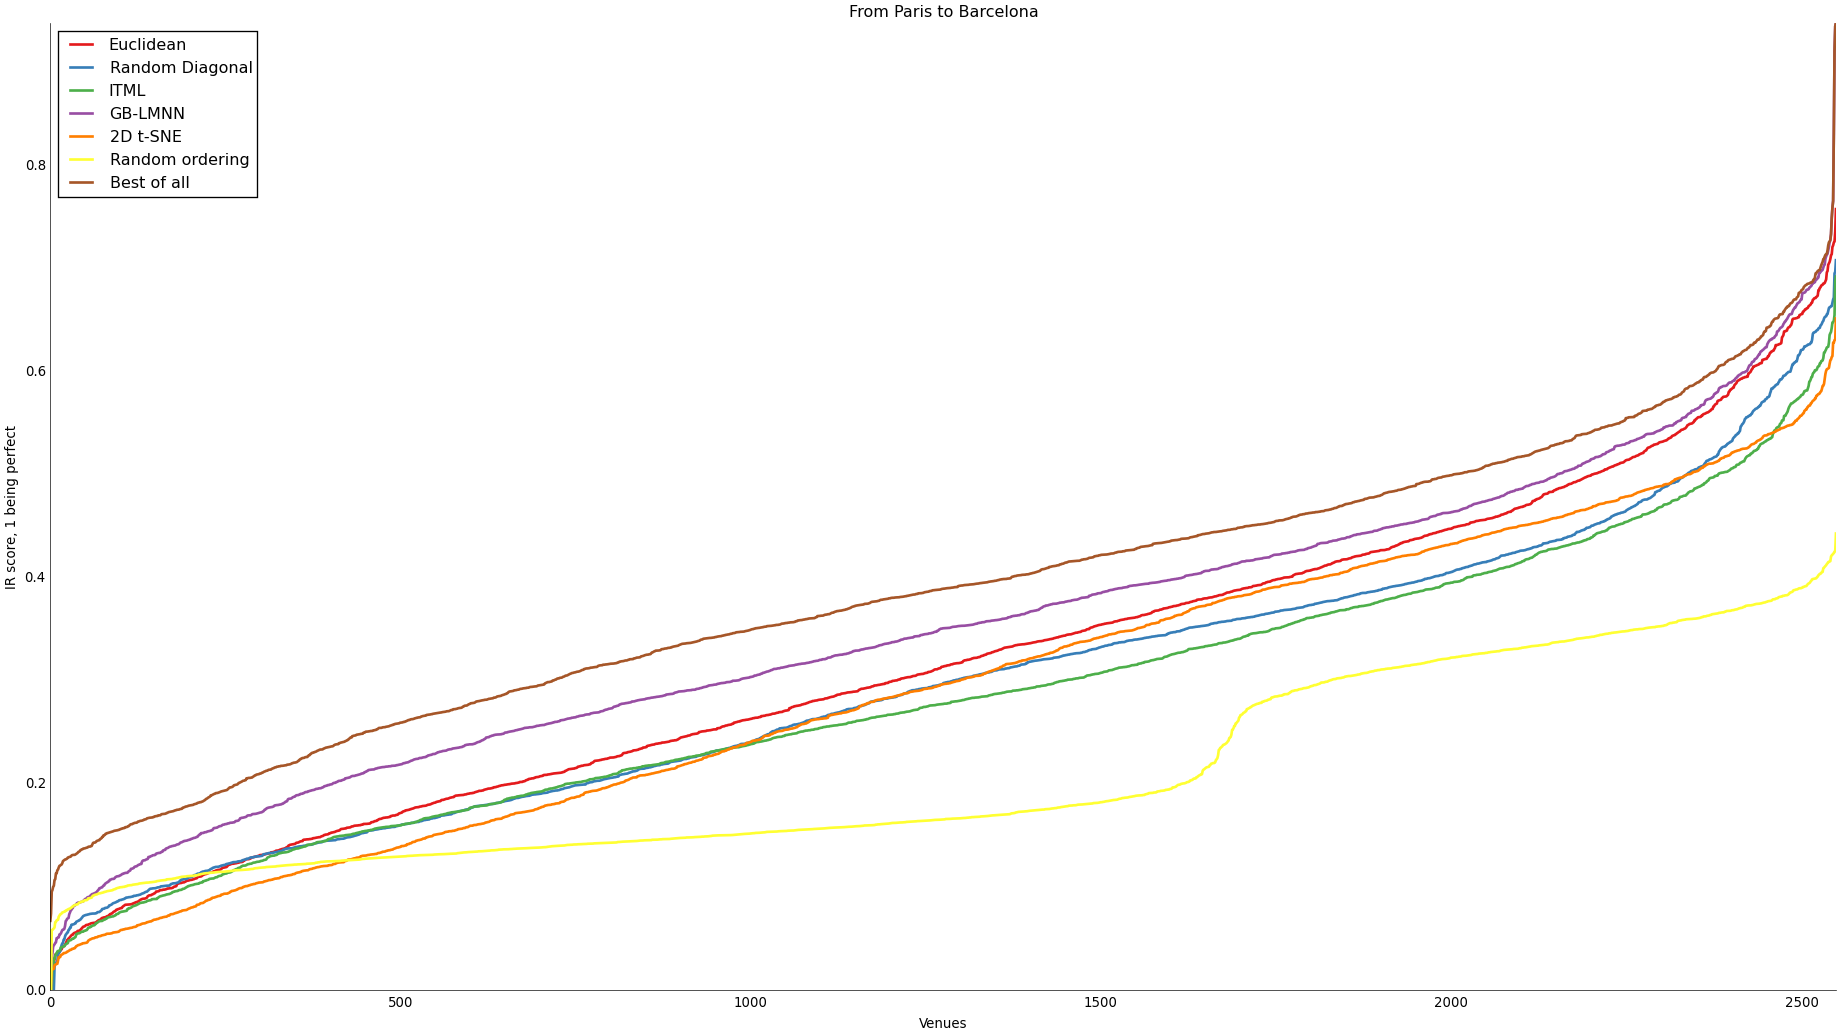
\includegraphics[width=\linewidth]{ir_paris_barca_sorted}
        \caption{The DCG score of each venues, sorted for all metrics.}
    \end{subfigure}

    \begin{subfigure}[b]{\textwidth}
        \centering
        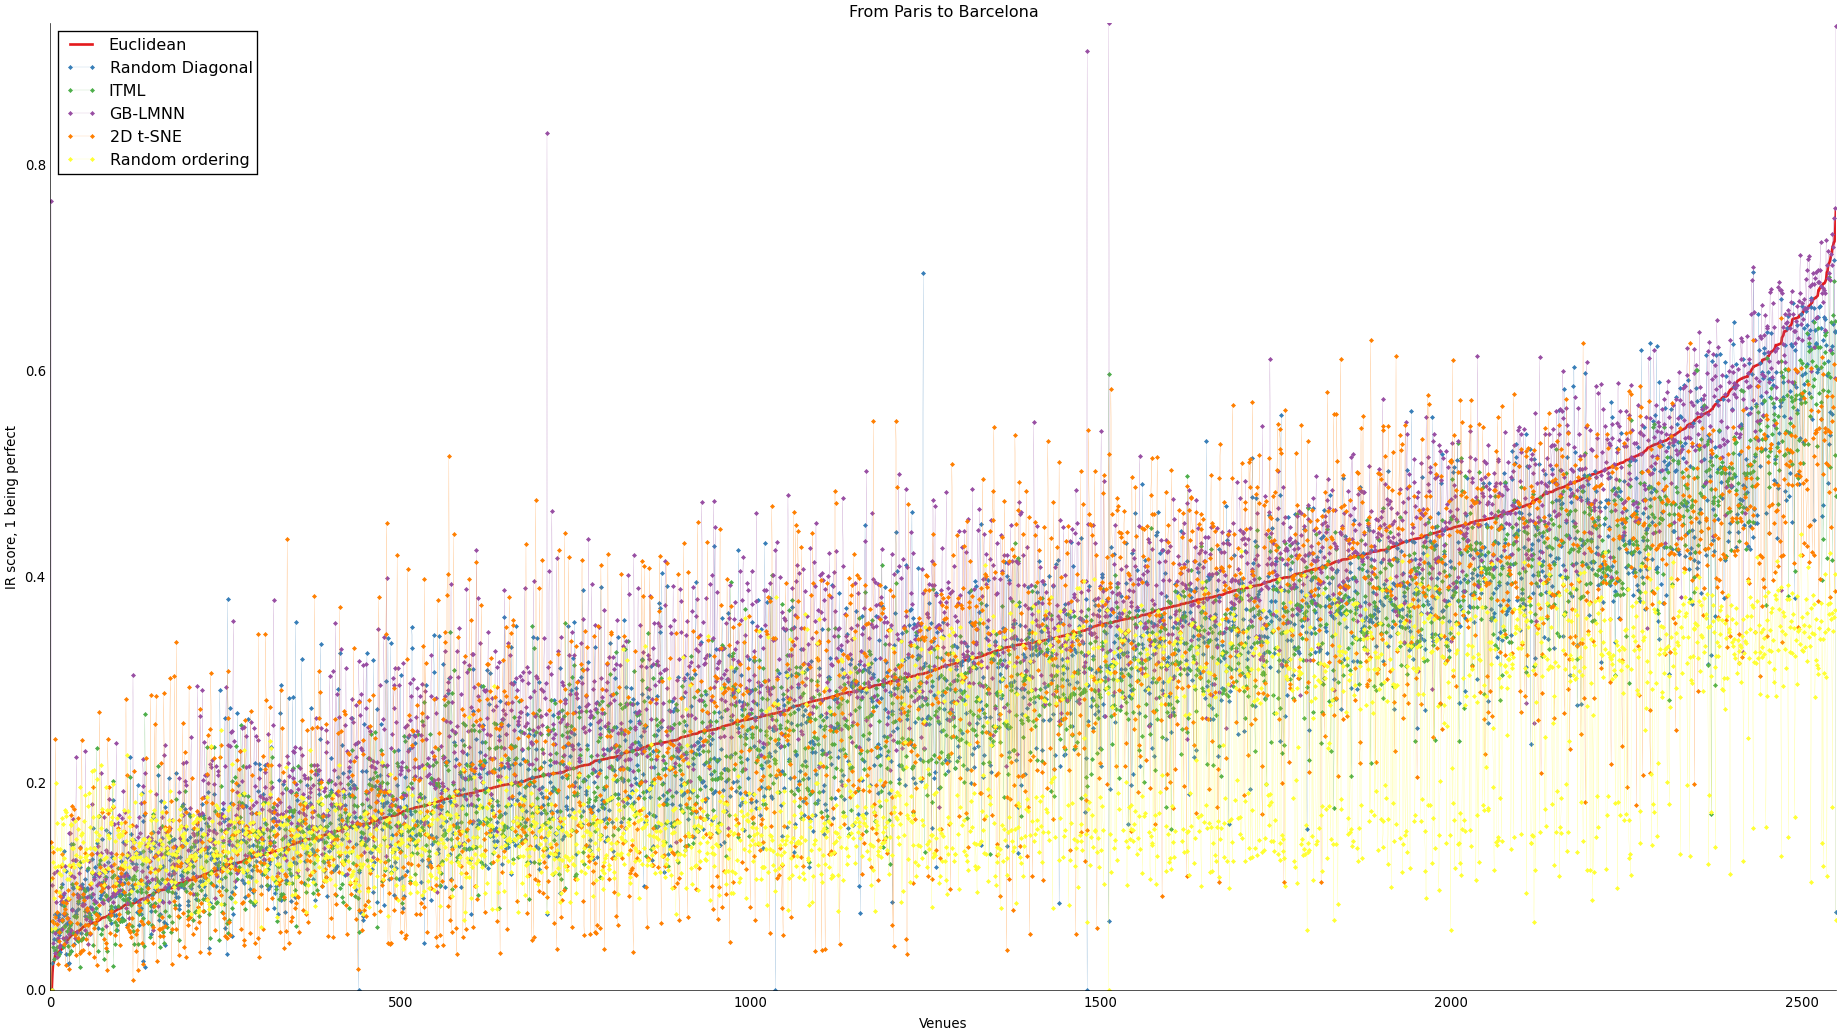
\includegraphics[width=\linewidth]{ir_paris_barca_raw}
        \caption{The DCG score of each venues, sorted by one metric.}
    \end{subfigure}
    \caption{Matching venues category.\label{fig:category}}
\end{figure}

\section{Neighborhoods metrics}

As mentioned in the background, the first metric we consider is EMD. More
precisely, three variants of it: Euclidean ground metric, LMNN-learned ground
metric and 80\%-EMD. In the last case, we reformulate the linear problem so
that only 80\% of the probability mass has to be moved from one distribution
to the other and we solve it with MATLAB.  Specifically, if we have
distribution $P$ and $Q$ with weights $w_P$ and $w_Q$ summing to one and a ground metric $d$
between them, we find the flow $f$ solving:
\begin{align*}
	&\quad \underset{f}{\min} \sum_{i,j} d_{i,j} f_{i,j} \\
	\text{subject to} &\quad \sum_j f_{i,j} \leq w_{P,i} \\
	&\quad \sum_i f_{i,j} \leq w_{Q,j} \\
	&\quad \sum_{i,j} f_{i,j} \geq 0.8 
\end{align*}

Then we used JSD. As it is based on Kullback--Leibler divergence, it can be
computed for multivariate distribution. But because our samples are small --
typically a neighborhood contains around 100 venues, and never more than 700 --
it was not possible to accurately estimate the probability density function.
There are some workarounds \autocite{EstimateKL07} but instead, we estimate the
density of each feature $p_i$ and $q_i$ independently\footnote{With a simple
10-bins histogram.}, compute their JSD $J_{P,Q}^i = JSD(p_i, q_i)$ and take a
weighted combination of the results $d_{JSD}(P, Q) = \sum_i\theta_i J_{P,Q}^i$.
We choose $\theta$ such that it gives small distance between related ground
regions and a large one between the others. Formally, we have 102 regions with
at least 9 venues inside. For each pair, we put $J_{P,Q}$ in one row a matrix
$D$ and we assign a $\pm 1$ label, depending of whether regions $P$ and $Q$ are
in the same class or not. We want to minimize $\sum_{y_{P,Q} = 1} d_{JSD}(P, Q)
- \sum_{y_{P,Q} = -1} d_{JSD}(P, Q)$ so we multiply each row of $D$ by
$\frac{y_{P,Q}}{|\{y,\, y = y_{P,Q}\}|}$ and solve $\min D\theta$ under the
constraints that $\theta$ is a positive unit norm vector whose coordinates are
lower bounded by 0.03 (to avoid the optimal zero solution)\footnote{I also
tried RankSVM but did not really use the result}. 

Finally we consider a simple baseline that draws on the same general ideas.
Given a query area, we cluster the venues inside using Euclidean distance in
the features space. We do the same in the other region and the distance is the
minimal cost of the assignment problem between these two sets of three
centroids.


All these methods can accept weighted input. We consider using number of unique
visitors and thus paying more attention to popular venues but it did not
perform better.

\subsection{Evaluation}

Then we need to decide which of these metric is for apt to recover the ground
truth. Let say we have a region query (from one city) and a target city with
$n$ venues:  this define a query \textsf{(city, district)} associated with
$\{g_1, \ldots, g_n\}$ known relevant results (each $g_i$ is a ground truth
polygon defined by a human judge, with a least 20 venues inside). Furthermore,
we have infinite computational power. There are at most $\sum_i \binom{n}{i}$
polygons defined by these $n$ venues. We remove those that do not form
neighborhoods (because they are made of several parts or they have holes
inside) and compute the distance to the query for the remaining ones. By
selecting the $m$ non-overlapping of them with the smallest distance, we get a
list of results $\{r_1, \ldots, r_m\}$ that the most similar neighborhood to
the query according to the metric at hand. We can then asses how well this
match the ground truth.

To alleviate the irritating lack of infinite power, we restrict our polygons to
be circle of radius $\{200, 275, 350, 425, 500\}$ meters, whose centers are set
on a regular grid over the city and we keep the $m = 5$ disjoint circles with
the smallest distance.

The relevance of each result list is computed as 
\[ rel_i = \max_{g_j} rel(r_i, g_j) \]
where
\[ rel(r_i, g_j) = \frac{| V_r \cap V_g|}{|V_r \cup V_g|} \]
is the Jaccard similarity between set of venues.

Like before, we used Discounted Cumulative Gain as a measure of quality. This
time though, there is no normalization, as the ideal score would be the same
for every metric and would thus not affect their relative order. Each city is
the query city in turn. For each district, we choose a representative region
(that have at least 20 venues within and in case of several candidates, the
closest to 150 venues). In each target city, we retrieve gold regions $g_1,
\ldots, g_n$.
This gives $Q$ queries \[
	Q \leq \underbrace{6}_{\text{target cities}} \times
	\underbrace{8}_{\text{districts}} \]

and we compute the average score \[
\mathrm{ADCG_{m}} = \frac{1}{Q}\sum_{q=1}^Q \sum_{i=1}^m \frac{ 2^{rel_{i}} - 1 }{\log_{2}(i+1)}
\]

The results are shown in \autoref{tab:cmp_metric}~\vpageref{tab:cmp_metric} and
according to them, we choose plain EMD, while noting that JSD performs rather
poorly.

\begin{table}[ht]
    \centering
\begin{tabular}{lccccc}
\toprule
              & Cluster  & EMD      & EMD-LMNN & JSD      & 80\%-EMD\\% & Average \\
\midrule
Barcelona     & 0.083064 & 0.078173 & \cbest{0.084204} & 0.042414 & 0.078244\\% & \textit{0.073220} \\
New York      & 0.059200 & \cbest{0.059385} & 0.059023 & 0.057180 & 0.053495\\% & \textit{0.057656} \\
Paris         & 0.061438 & \cbest{0.091178} & 0.078614 & 0.045136 & 0.061940\\% & \textit{0.067661} \\
Rome          & 0.024313 & \cbest{0.042352} & 0.039936 & 0.021156 & 0.029746\\% & \textit{0.031501} \\
San Francisco & \cbest{0.045977} & 0.045031 & 0.040164 & 0.033829 & 0.044497\\% & \textit{0.041899} \\
Washington    & \cbest{0.043694} & 0.034762 & 0.038164 & 0.033211 & 0.038829\\% & \textit{0.037732} \\
Average       & \textit{0.052947} & \textit{\cbest{0.058480}} & \textit{0.056684} & \textit{0.038821} & \textit{0.051125}\\% & \textit{0.051612} \\
\bottomrule
\end{tabular}
\caption[Average score of each metric]{Average score of each metric when query
        are issued from the city on the left. The best metric in each city is
        \cbest{highlighted} and the last row is the average score over all
        cities.\label{tab:cmp_metric}}
\end{table}
